\section{Introduction}
\label{kvdirect:sec:introduction}

The theme of this chapter is storage virtualization and data structure processing acceleration, as shown in Figure \ref{kvdirect:fig:sys-arch}. Among them, data structure processing acceleration is the focus of this article, and storage virtualization is only briefly discussed in Section \ref{sec:durable-storage}.

\begin{figure}[htbp]
	\centering
	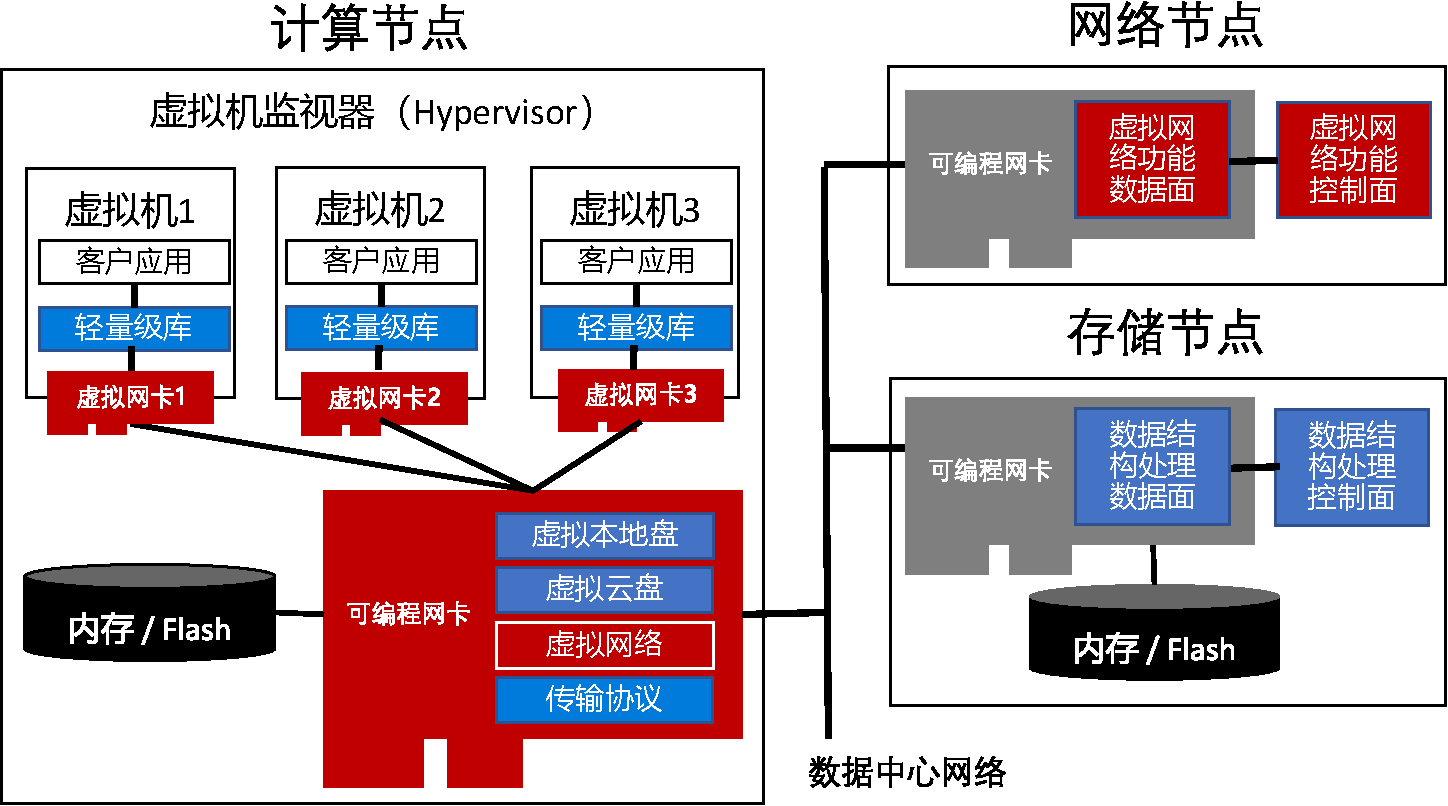
\includegraphics[width=0.8\textwidth]{figure/sys_arch.pdf}
	\caption{The theme of this chapter: storage virtualization and data structure processing acceleration, marked with a bold oblique line background.}
	\label{kvdirect:fig:sys-arch}
\end{figure}

In terms of programmable network card programming, this chapter builds on the ClickNP programming framework proposed in the previous chapter, establishes the foundation of the service layer, proposes a framework for stateful processing and data structure processing, and implements memory key-value storage based on this, as shown in Figure \ref{kvdirect:fig:sw-hw-codesign}.

\begin{figure}[htbp]
	\centering
	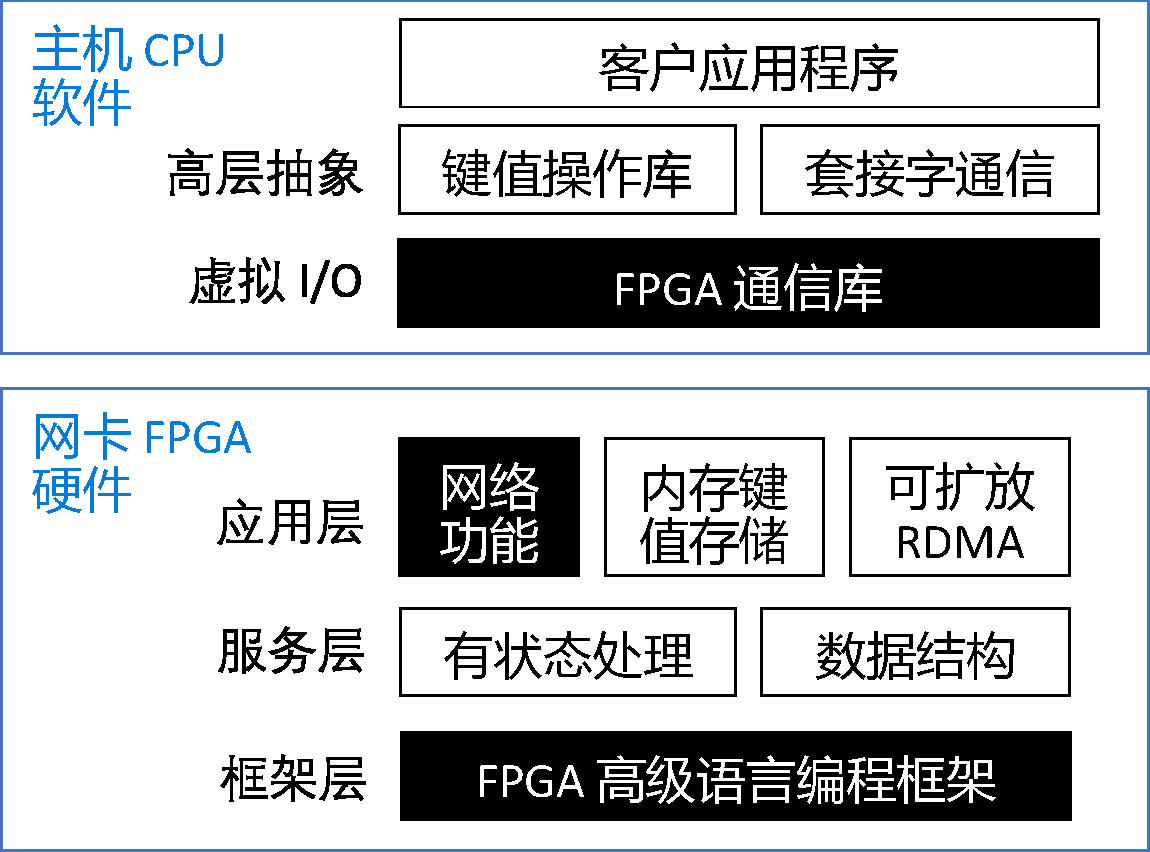
\includegraphics[width=0.5\textwidth]{figure/sw_hw_codesign.pdf}
	\caption{The position of this chapter in the programmable network card software and hardware architecture.}
	\label{kvdirect:fig:sw-hw-codesign}
\end{figure}

In-memory key-value storage is a key component of distributed systems in data centers. This chapter presents \oursys{}, an in-memory key-value system based on programmable network cards. As the name suggests, the programmable network card of \oursys{} receives and processes key-value operation requests from the network, and applies updates directly in the host memory, bypassing the host CPU. \oursys{} extends RDMA primitives from memory operations (read and write) to key-value operations (GET, PUT, DELETE, and atomic operations). Furthermore, to support vector-based operations and reduce network traffic, \oursys{} also provides new vector primitives UPDATE, REDUCE, and FILTER, allowing users to define active messages \cite {eicken1992active} and delegate certain computations to the programmable network card.

The design focus of key-value processing within the programmable network card is to optimize PCIe traffic between the network card and the host memory. \oursys{} adopts a series of optimizations to fully utilize PCIe bandwidth and hide latency. Firstly, \oursys{} designs a new hash table and memory allocator to take advantage of FPGA's parallelism and minimize the number of PCIe DMA requests. On average, \oursys{} uses only close to one PCIe DMA operation per GET operation and two PCIe DMA operations per PUT operation. Secondly, to ensure the consistency of key-value storage, \oursys{} designs an out-of-order execution engine to track operation dependencies while maximizing the throughput of independent requests. Thirdly, \oursys{} implements a hardware-based load dispatcher and cache components in FPGA to fully utilize the bandwidth and capacity of onboard DRAM.

Based on the above optimization, a single network card \oursys{} system can achieve up to 180~M key-value operations per second, equivalent to the throughput of 36 CPU cores \cite {li2016full}.
Compared with the most advanced CPU key-value storage system, \oursys{} can reduce tail latency to 10 $\mu$s, while improving energy efficiency by 3 times.
Moreover, \oursys{} can achieve near-linear scalability through multiple network cards. By using 10 programmable network cards in a single commodity server, the performance can reach 1.22 billion key-value operations per second, which is an order of magnitude higher than existing systems.

\oursys{} also supports up to 180~Mops of general atomic operations, significantly better than the performance reported in the most advanced RDMA-based systems: 2.24~Mops \cite {kalia2014using}. The high performance of atomic operations is mainly attributed to the out-of-order execution engine. The out-of-order execution engine can efficiently track dependencies between key-value operations without blocking the pipeline.

The rest of this chapter is arranged as follows. Section \ref {kvdirect:sec:background} introduces the background, and clarifies the design goals and challenges.
Section \ref {kvdirect:sec:architecture} describes the design of \oursys{}.
Section \ref {kvdirect:sec:evaluation} evaluates the performance of \oursys{}.
Sections \ref {kvdirect:sec:extensions} and \ref {kvdirect:sec:discussion} discuss the extensions of this paper.
Section \ref {kvdirect:sec:related} discusses related work.
Section \ref {kvdirect:sec:conclusion} concludes.
